\documentclass[conference]{IEEEtran}
\IEEEoverridecommandlockouts
\usepackage{cite}
\usepackage{amsmath,amssymb,amsfonts}
\usepackage{graphicx}
\usepackage{textcomp}
\usepackage{xcolor}
\usepackage{booktabs}
\usepackage{multirow}
\usepackage{tikz}
\usetikzlibrary{arrows.meta,positioning,calc}
\graphicspath{{figs/}}
% auto-generated by make_figures.py from results/metrics.json -- do not edit
\newcommand{\nTest}{600}
\newcommand{\mainName}{Ours (final)}
\newcommand{\psnrSarGray}{9.86}
\newcommand{\ssimSarGray}{0.037}
\newcommand{\samSarGray}{9.41}
\newcommand{\gmsdSarGray}{0.261}
\newcommand{\psnrMeanColor}{13.96}
\newcommand{\ssimMeanColor}{0.238}
\newcommand{\samMeanColor}{9.88}
\newcommand{\gmsdMeanColor}{0.288}
\newcommand{\psnrUnetLB}{14.14}
\newcommand{\ssimUnetLB}{0.237}
\newcommand{\samUnetLB}{11.23}
\newcommand{\gmsdUnetLB}{0.274}
\newcommand{\psnrPixCpix}{12.58}
\newcommand{\ssimPixCpix}{0.149}
\newcommand{\samPixCpix}{16.96}
\newcommand{\gmsdPixCpix}{0.241}
\newcommand{\psnrLeePixCpix}{12.64}
\newcommand{\ssimLeePixCpix}{0.133}
\newcommand{\samLeePixCpix}{12.42}
\newcommand{\gmsdLeePixCpix}{0.247}
\newcommand{\psnrOursNodesp}{12.55}
\newcommand{\ssimOursNodesp}{0.153}
\newcommand{\samOursNodesp}{14.07}
\newcommand{\gmsdOursNodesp}{0.250}
\newcommand{\psnrOursNophys}{12.54}
\newcommand{\ssimOursNophys}{0.173}
\newcommand{\samOursNophys}{16.67}
\newcommand{\gmsdOursNophys}{0.253}
\newcommand{\psnrOurs}{12.14}
\newcommand{\ssimOurs}{0.161}
\newcommand{\samOurs}{14.45}
\newcommand{\gmsdOurs}{0.249}
\newcommand{\psnrOursCond}{11.84}
\newcommand{\ssimOursCond}{0.156}
\newcommand{\samOursCond}{14.27}
\newcommand{\gmsdOursCond}{0.252}
\newcommand{\psnrOursCondnolabel}{12.45}
\newcommand{\ssimOursCondnolabel}{0.152}
\newcommand{\samOursCondnolabel}{13.70}
\newcommand{\gmsdOursCondnolabel}{0.251}
\newcommand{\psnrOursNoadv}{14.47}
\newcommand{\ssimOursNoadv}{0.247}
\newcommand{\samOursNoadv}{11.74}
\newcommand{\gmsdOursNoadv}{0.279}
\newcommand{\psnrOursRBICondNoadv}{14.33}
\newcommand{\ssimOursRBICondNoadv}{0.248}
\newcommand{\samOursRBICondNoadv}{11.81}
\newcommand{\gmsdOursRBICondNoadv}{0.278}
\newcommand{\psnrOursRBICondNoadvnolabel}{14.55}
\newcommand{\ssimOursRBICondNoadvnolabel}{0.249}
\newcommand{\samOursRBICondNoadvnolabel}{11.26}
\newcommand{\gmsdOursRBICondNoadvnolabel}{0.279}
\newcommand{\psnrOurspluslum}{14.37}
\newcommand{\ssimOurspluslum}{0.233}
\newcommand{\samOurspluslum}{11.65}
\newcommand{\gmsdOurspluslum}{0.269}
\newcommand{\psnrOursplusdetail}{14.33}
\newcommand{\ssimOursplusdetail}{0.242}
\newcommand{\samOursplusdetail}{11.91}
\newcommand{\gmsdOursplusdetail}{0.276}
\newcommand{\enlRaw}{39.4}
\newcommand{\epiRaw}{1.000}
\newcommand{\morRaw}{1.000}
\newcommand{\enlLee}{171.7}
\newcommand{\epiLee}{0.858}
\newcommand{\morLee}{0.988}
\newcommand{\enlOursNophys}{14.7}
\newcommand{\epiOursNophys}{0.608}
\newcommand{\morOursNophys}{1.348}
\newcommand{\enlOurs}{43.9}
\newcommand{\epiOurs}{0.599}
\newcommand{\morOurs}{0.997}
\newcommand{\enlOursCond}{52.1}
\newcommand{\epiOursCond}{0.659}
\newcommand{\morOursCond}{0.995}
\newcommand{\enlOursNoadv}{49.5}
\newcommand{\epiOursNoadv}{0.624}
\newcommand{\morOursNoadv}{0.998}
\newcommand{\enlOursRBICondNoadv}{54.7}
\newcommand{\epiOursRBICondNoadv}{0.903}
\newcommand{\morOursRBICondNoadv}{0.986}
\newcommand{\ause}{0.0675}
\newcommand{\uncRho}{0.005}
\newcommand{\mcT}{10}
\newcommand{\mcGain}{+0.02}
\newcommand{\nMC}{160}
\newcommand{\dGanCost}{2.34}
\newcommand{\dPixVsUnet}{1.57}
\newcommand{\dFinalVsUnet}{0.18}
\newcommand{\dFinalVsPix}{1.75}
\newcommand{\dFinalVsMean}{0.37}
\newcommand{\dNoLabelVsUnet}{0.40}
\newcommand{\dNoLabelVsFinal}{0.22}
\newcommand{\dSsimFinalVsUnet}{0.011}
\newcommand{\pFinalUnetPsnr}{0.013}
\newcommand{\pFinalUnetSsim}{\ensuremath{<10^{-13}}}
\newcommand{\pFinalUnetSam}{0.614}
\newcommand{\pFinalPixPsnr}{\ensuremath{<10^{-60}}}
\newcommand{\pFinalMeanPsnr}{\ensuremath{<10^{-5}}}
\newcommand{\pNoLabelPsnr}{\ensuremath{<10^{-7}}}
\newcommand{\fusionAlpha}{0.1}
\newcommand{\fusionBeta}{0.25}
   % every number below is generated from results/metrics.json

% From the official IEEE conference template: start a second row of authors.
\makeatletter
\newcommand{\linebreakand}{%
  \end{@IEEEauthorhalign}
  \hfill\mbox{}\par
  \mbox{}\hfill\begin{@IEEEauthorhalign}
}
\makeatother

\begin{document}

\title{Physics-Guided SAR-to-Optical Colorization with Radiometry-Preserving Despeckling: A Leakage-Free Benchmark on Sentinel-1/2}

\author{
\IEEEauthorblockN{Selvanayaki S}
\IEEEauthorblockA{\textit{Dept. of Artificial Intelligence and Data Science}\\
\textit{Saveetha Engineering College}\\ Chennai, India \\ selvanayakis@saveetha.ac.in}
\and
\IEEEauthorblockN{Dr. K. Micheal Mahesh}
\IEEEauthorblockA{\textit{Dept. of Electronics and Communication Engineering}\\
\textit{Saveetha Engineering College}\\ Chennai, India \\ michealmaheshk@saveetha.ac.in}
\and
\IEEEauthorblockN{Kolli Amos Daniel}
\IEEEauthorblockA{\textit{Dept. of Artificial Intelligence and Machine Learning}\\
\textit{Saveetha Engineering College}\\ Chennai, India \\ kollihimantharao@saveetha.ac.in}
\linebreakand
\IEEEauthorblockN{Gedipudi Darshani}
\IEEEauthorblockA{\textit{Dept. of Artificial Intelligence and Data Science}\\
\textit{Saveetha Engineering College}\\ Chennai, India \\ gedipudidarshani@gmail.com}
\and
\IEEEauthorblockN{Yenuganti Prathyusha}
\IEEEauthorblockA{\textit{Dept. of Artificial Intelligence and Machine Learning}\\
\textit{Saveetha Engineering College}\\ Chennai, India \\ yenugantiprathyusharavi@gmail.com}
\and
\IEEEauthorblockN{P Keerthana}
\IEEEauthorblockA{\textit{Dept. of Artificial Intelligence and Machine Learning}\\
\textit{Saveetha Engineering College}\\ Chennai, India \\ keerthanap816@gmail.com}
}

\maketitle

\begin{abstract}
Synthetic Aperture Radar (SAR) images the Earth through cloud and at night, but its single-channel, speckled backscatter
is hard for non-experts to interpret. We study SAR-to-optical colorization with a two-stage, physics-guided network.
Stage~1 is a log-domain (homomorphic) residual despeckler that is trained \emph{without clean references}. It is supervised
by a prior derived from the multiplicative speckle model: local radiometric preservation plus log-domain total variation.
Stage~2 is a U-Net colorizer with an ImageNet-pretrained ResNet-18 encoder and terrain-conditioned FiLM layers. We evaluate on
16{,}000 Sentinel-1/Sentinel-2 pairs with a \emph{scene-level} split, so no test scene is seen in training, and train nine
models (baselines and ablations) under an identical budget. On \nTest{} test tiles the final model reaches \psnrOursRBICondNoadv{}\,dB
PSNR and \ssimOursRBICondNoadv{} SSIM. That is \dFinalVsPix{}\,dB above Pix2Pix and \dFinalVsUnet{}\,dB above a U-Net regressor,
a difference that is statistically significant under a paired Wilcoxon test. The physics prior makes Stage~1 radiometrically
unbiased (mean of ratio \morOurs{} versus \morOursNophys{} without it). We also report three negative results: the adversarial loss
costs \dGanCost{}\,dB on unseen scenes; terrain conditioning does not transfer across scenes; and Monte Carlo dropout variance does
not rank pixel errors (Spearman correlation \uncRho{}). The absolute scores show that colorizing unseen scenes from
single-polarization SAR remains far from solved. Code, splits and evaluation scripts are released.
\end{abstract}

\begin{IEEEkeywords}
Synthetic aperture radar, image colorization, despeckling, Sentinel-1, Sentinel-2, image-to-image translation, uncertainty.
\end{IEEEkeywords}

\section{Introduction}
Optical satellites such as Sentinel-2 cannot image the ground through cloud, smoke or at night, which is often exactly when
imagery is needed for disaster response. Synthetic Aperture Radar (SAR) such as Sentinel-1 is an active microwave sensor
that works in all weather, day and night~\cite{torres2012s1}. Its output, however, is a single-channel backscatter image
corrupted by multiplicative speckle~\cite{goodman1976speckle}, and it is hard to read for anyone who is not a radar
specialist. Translating SAR into an optical-like colour image is therefore attractive and is the subject of the ISRO
Smart India Hackathon problem SIH1733, ``SAR Image Colorization for Comprehensive Insight using Deep Learning''.

Most published approaches treat the task as generic image-to-image translation with conditional or cycle-consistent
GANs~\cite{isola2017pix2pix,zhu2017cyclegan,wang2019sar2opt,fuentes2019sar2opt}. One network then has to suppress speckle and
infer colour at the same time, with no model of how speckle is formed. The translation is also fundamentally ambiguous: the
same backscatter can correspond to many optical appearances. In addition, evaluations often draw training and test patches
from the same scenes. Overlapping patches then leak between the splits, and the scores come out optimistic.

Our contributions are:
\begin{itemize}
\item A two-stage generator whose first stage is a homomorphic despeckler trained \emph{without clean SAR references}. It is
supervised by a physics prior derived from the speckle model, and we show that this prior removes a large radiometric bias
that the stage otherwise develops.
\item A leakage-free, scene-level benchmark on 16{,}000 Sentinel-1/2 pairs. Nine models (three baselines and six variants of ours)
plus two trivial floors are compared, all trained under an identical budget and compared with paired significance tests.
\item Controlled evidence that, on unseen scenes, the adversarial loss lowers PSNR by about 2\,dB and the non-adversarial
physics-guided models perform best, significantly ahead of Pix2Pix and a U-Net regressor.
\item Three negative results that we report rather than omit: terrain conditioning, Monte Carlo dropout uncertainty, and SAR
luminance fusion do not deliver the gains commonly assumed.
\end{itemize}
All code, the split file and the evaluation scripts are released so that every number can be reproduced.

\section{Related Work}
\textbf{SAR-to-optical translation.} Pix2Pix~\cite{isola2017pix2pix} couples an L1 loss with a PatchGAN discriminator, and
CycleGAN~\cite{zhu2017cyclegan} removes the need for paired data. Both have been adapted to SAR~\cite{wang2019sar2opt,fuentes2019sar2opt}.
Fuentes Reyes \emph{et al.}~\cite{fuentes2019sar2opt} observe that such models produce plausible textures but unreliable colours
on unseen scenes, and our benchmark quantifies this effect. Natural-image colorization~\cite{zhang2016colorful} relies on semantic
priors that do not transfer to radar.

\textbf{Despeckling.} The Lee filter~\cite{lee1980filter} uses local statistics, and total-variation methods~\cite{rudin1992tv}
favour piecewise-smooth solutions. CNN despecklers~\cite{chierchia2017sarcnn} use residual learning~\cite{zhang2017dncnn} in the
log domain but normally need clean or multi-temporal references. Our Stage~1 learns from a physics prior instead, jointly with
the colorization objective.

\textbf{Uncertainty.} MC dropout~\cite{gal2016dropout} approximates Bayesian inference by sampling dropout masks at test time
and targets epistemic uncertainty~\cite{kendall2017uncertainty}. Sparsification analysis~\cite{ilg2018uncertainty} tests
whether that uncertainty actually ranks pixels by their error.

\section{Method}
Fig.~\ref{fig:arch} shows the pipeline.
\begin{figure*}[t]
\centering
% Architecture diagram (TikZ) -- compiled inline, no external image needed.
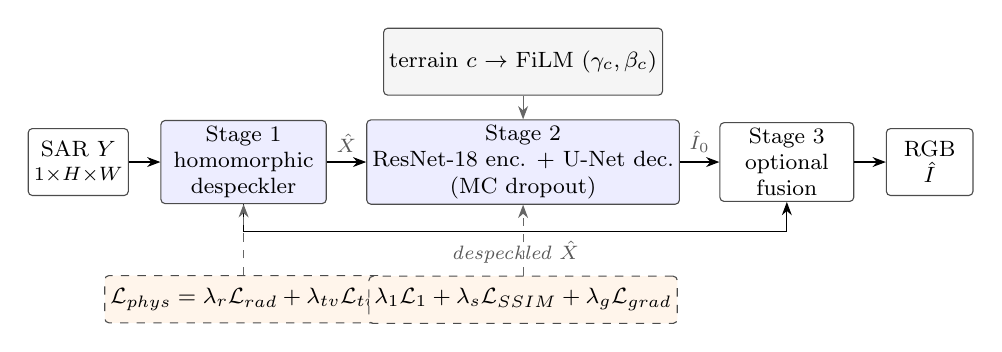
\begin{tikzpicture}[
  font=\footnotesize, >=Stealth, node distance=3mm,
  box/.style={draw=black!70, rounded corners=1.5pt, align=center, minimum height=8.5mm, inner sep=2pt, fill=white},
  stage/.style={box, fill=blue!7},
  loss/.style={box, dashed, fill=orange!8, minimum height=6mm},
  lab/.style={font=\scriptsize\itshape, text=black!65}]
  \node[box, minimum width=12mm] (y) {SAR $Y$\\[-1pt]\scriptsize $1{\times}H{\times}W$};
  \node[stage, right=4mm of y, minimum width=21mm] (s1) {Stage 1\\homomorphic\\despeckler};
  \node[stage, right=5mm of s1, minimum width=27mm] (s2) {Stage 2\\ResNet-18 enc. + U-Net dec.\\(MC dropout)};
  \node[box, right=5mm of s2, minimum width=17mm] (fu) {Stage 3\\optional\\fusion};
  \node[box, right=4mm of fu, minimum width=11mm] (out) {RGB\\$\hat{I}$};
  \draw[->] (y) -- (s1);
  \draw[->] (s1) -- node[above, lab]{$\hat X$} (s2);
  \draw[->] (s2) -- node[above, lab]{$\hat I_{0}$} (fu);
  \draw[->] (fu) -- (out);
  \draw[->] (s1.south) -- ++(0,-3.5mm) -| node[pos=0.25, below, lab]{despeckled $\hat X$} (fu.south);
  \node[box, above=3mm of s2, minimum width=27mm, fill=black!4] (film) {terrain $c$ $\rightarrow$ FiLM $(\gamma_c,\beta_c)$};
  \draw[->, black!60] (film.south) -- (s2.north);
  \node[loss, below=9mm of s1, minimum width=26mm] (lp) {$\mathcal{L}_{phys}=\lambda_{r}\mathcal{L}_{rad}+\lambda_{tv}\mathcal{L}_{tv}$};
  \node[loss, below=9mm of s2, minimum width=30mm] (lc) {$\lambda_1\mathcal{L}_1+\lambda_s\mathcal{L}_{SSIM}+\lambda_g\mathcal{L}_{grad}$};
  \draw[->, dashed, black!60] (lp) -- (s1);
  \draw[->, dashed, black!60] (lc) -- (s2);
\end{tikzpicture}

\caption{Proposed pipeline. Stage~1 removes speckle in the log domain and is supervised by the physics prior $\mathcal{L}_{phys}$.
Stage~2 predicts RGB from the despeckled image and is modulated by a terrain embedding (FiLM). Stage~3 optionally injects SAR
detail. Repeated stochastic passes through the decoder dropout layers give a predictive mean and variance.}
\label{fig:arch}
\end{figure*}

\subsection{Speckle model and Stage 1}
The observed intensity is modelled as $Y = X\cdot F$, where $X$ is the reflectivity and $F$ is speckle with
$\mathbb{E}[F]=1$~\cite{goodman1976speckle}. In the log domain this becomes additive, $\log Y = \log X + \log F$. Stage~1 is a
residual CNN (a $3{\times}3$ convolution, two residual blocks of 64 channels, and a $\tanh$-bounded output) that predicts
$\widehat{\log F}$ and returns $\hat X = \exp(\log Y - \widehat{\log F})$. No clean reflectivity is available, so Stage~1 is
supervised by two properties of the speckle model:
\begin{align}
\mathcal{L}_{rad} &= \big\| \mathcal{A}_w(\hat X) - \mathcal{A}_w(Y) \big\|_1, \label{eq:rad}\\
\mathcal{L}_{tv}  &= \big\| \nabla \log(\hat X+\epsilon) \big\|_1, \label{eq:tv}
\end{align}
where $\mathcal{A}_w$ is a $w{\times}w$ moving average ($w{=}7$). Because $\mathbb{E}[Y]=X$, the local multi-look mean of $Y$
is an unbiased estimate of $X$, so (\ref{eq:rad}) forbids the despeckler from changing the radiometry. Term (\ref{eq:tv}) is a
log-domain total-variation prior~\cite{rudin1992tv} that penalises the high-frequency, additive $\log F$.

\subsection{Stage 2: colorization}
The colorizer is a U-Net~\cite{ronneberger2015unet}. Its encoder is the stem and first three stages of an ImageNet-pretrained
ResNet-18. The despeckled SAR is replicated to three channels and normalised with ImageNet statistics before entering the
encoder. A $16{\times}16$ bottleneck feeds a decoder that uses bilinear upsampling (to avoid checkerboard artefacts) and spatial
dropout with $p=0.15$, $0.10$ and $0.05$. The output layer also receives $\hat X$ through a skip connection.

\textbf{Terrain FiLM.} A learned embedding of the terrain class $c\in\{$agriculture, barren, grassland, urban$\}$ produces a
per-channel scale and shift $(\gamma_c,\beta_c)$~\cite{perez2018film}. These modulate the bottleneck and three decoder levels as
$h\mapsto h\,(1+\gamma_c)+\beta_c$. The embedding is zero-initialised, so training starts from the unconditioned network. A
fifth, ``unknown'' embedding is trained by replacing the label with probability 0.2, so the model also runs without a label.

\textbf{Loss.} The generator minimises
\begin{equation}
\mathcal{L} = \lambda_1\mathcal{L}_1 + \lambda_s(1-\mathrm{SSIM}) + \lambda_g\mathcal{L}_{grad} + \lambda_a\mathcal{L}_{GAN}
+ \lambda_r\mathcal{L}_{rad} + \lambda_{tv}\mathcal{L}_{tv},
\end{equation}
where $\mathcal{L}_{grad}$ is the L1 distance between the image gradients of the prediction and of the target, and
$\mathcal{L}_{GAN}$ uses a PatchGAN discriminator conditioned on the SAR input~\cite{isola2017pix2pix}. We use
$\lambda_1{=}100$, $\lambda_s{=}10$, $\lambda_g{=}10$, $\lambda_r{=}10$ and $\lambda_{tv}{=}0.5$. Our first version used
$\lambda_a{=}1$. The final model uses $\lambda_a{=}0$, a choice made on the validation scenes (Section~\ref{sec:ablation}).

\subsection{Stage 3: optional structure-guided fusion}
The prediction is converted to CIELAB. \emph{Luminance replacement} sets $L^* = \alpha S + (1-\alpha)L^*_{pred}$, where $S$ is
the percentile-stretched $\hat X$. \emph{Detail injection}, in the spirit of component-substitution
pansharpening~\cite{vivone2015pansharp}, adds only the high-pass part of the SAR:
$L^* = L^*_{pred} + \beta\,\frac{\sigma(L^*_{pred})}{\sigma(S)}\big(S - G_{\sigma} * S\big)$. In both cases the chroma $(a^*,b^*)$
is kept as predicted. The strengths $\alpha$ and $\beta$ are chosen on the validation scenes.

\subsection{Epistemic uncertainty}
At inference the batch-normalisation layers use their running statistics, and only the decoder dropout is sampled, over
$T{=}\mcT$ passes. This gives the predictive mean $\mu$ and the per-pixel variance $\sigma^2$, averaged over RGB.

\section{Experimental Setup}
\textbf{Data.} We use 16{,}000 co-registered Sentinel-1/Sentinel-2 pairs of $256{\times}256$ pixels derived from
SEN12MS~\cite{schmitt2019sen12ms}. They cover four terrain classes and 30 scenes. Sentinel-1 is given as 8-bit backscatter and
Sentinel-2 as 8-bit RGB~\cite{drusch2012s2}, and both are scaled to $[0,1]$.

\textbf{Leakage-free split.} Patches of one scene overlap and share appearance, so we split by \emph{scene}, with
stratification by class. This gives 11{,}014 training tiles (18 scenes), 1{,}139 validation tiles (4 scenes) and 3{,}847 test
tiles (8 scenes, all four classes). No scene appears in two splits, which an assertion in the split script enforces. We evaluate
a class-balanced subset of \nTest{} test tiles.

\textbf{Matched training budget.} Every model is trained with the same settings: 4{,}000 iterations, batch 8, random
$128{\times}128$ crops with flips and $90^\circ$ rotations, and Adam ($2{\times}10^{-4}$, $\beta_1{=}0.5$) with cosine decay,
in fp32 with seed 42 on one 2\,GB NVIDIA MX550 laptop GPU. Each model's checkpoint and the final configuration are selected by
validation L1. The test set is never used for any selection, including the fusion strengths and whether to supply the terrain
label. The baselines are a U-Net trained with L1 only, Pix2Pix~\cite{isola2017pix2pix}, and a Lee filter~\cite{lee1980filter}
($7{\times}7$, $L{=}40$, the median ENL of the training scenes) followed by Pix2Pix. Two trivial floors are also reported: the SAR
replicated as grey, and the mean training colour. We did not retrain CycleGAN, which targets unpaired data, or transformer and
diffusion models, which exceed our compute budget, and we do not copy their numbers from papers that use other data.

\textbf{Metrics.} We report PSNR, SSIM~\cite{wang2004ssim}, SAM~\cite{kruse1993sam} and GMSD~\cite{xue2014gmsd} (edge
fidelity) on full $256{\times}256$ tiles. Despeckling is assessed without a reference using three measures: ENL, computed on the
same homogeneous blocks of the raw and filtered image (median over tiles); EPI~\cite{sattar1997epi} relative to the raw SAR; and
the mean of the ratio image (MoR, ideal 1). Uncertainty is assessed with AUSE~\cite{ilg2018uncertainty} and with the Spearman
correlation between error and uncertainty. Every comparison with our final model uses the paired Wilcoxon signed-rank test.

\section{Results}
\subsection{Comparison with baselines}
Table~\ref{tab:main} and Fig.~\ref{fig:comparison} summarise the test results. The final model reaches \psnrOursRBICondNoadv{}\,dB
PSNR and \ssimOursRBICondNoadv{} SSIM. That is \dFinalVsPix{}\,dB above Pix2Pix ($p\,\pFinalPixPsnr$) and \dFinalVsUnet{}\,dB above
the U-Net regressor ($p=\pFinalUnetPsnr$), and SSIM is also higher (by \dSsimFinalVsUnet{}, $p\,\pFinalUnetSsim$). The SAM difference
from the U-Net is not significant ($p=\pFinalUnetSam$). Absolute scores are low for every method: the final model is only
\dFinalVsMean{}\,dB above predicting the mean training colour. This is the central practical finding. Colours in unseen scenes
depend on season, soil and vegetation state, and single-polarization backscatter alone does not determine them.

SAM must be read together with PSNR and SSIM. The trivial grey and mean-colour predictions obtain the \emph{lowest} SAM
(\samSarGray$^\circ$, \samMeanColor$^\circ$), because Sentinel-2 RGB in these scenes is close to neutral and SAM rewards
hue-neutral outputs regardless of their brightness.

\begin{table}[t]
\caption{Test results on \nTest{} tiles from scenes unseen in training (mean$\pm$std over tiles). Bold: best learned method.
$^\dagger$: not significantly different from Ours (final) (Wilcoxon $p\ge0.05$).}
\label{tab:main}
\centering\scriptsize\setlength{\tabcolsep}{3pt}
\resizebox{\columnwidth}{!}{\begin{tabular}{lcccc}
\toprule
Method & PSNR (dB)$\uparrow$ & SSIM$\uparrow$ & SAM ($^\circ$)$\downarrow$ & GMSD$\downarrow$ \\
\midrule
SAR as grey & 9.86$\pm$2.16 & 0.037$\pm$0.072 & 9.41$\pm$5.71 & 0.261$\pm$0.019 \\
Mean colour & 13.96$\pm$2.30 & 0.238$\pm$0.112 & 9.88$\pm$5.95 & 0.288$\pm$0.034 \\
\midrule
U-Net (L1) & 14.14$\pm$3.00 & 0.237$\pm$0.098 & \textbf{11.23}$\pm$6.23$^\dagger$ & 0.274$\pm$0.040 \\
Pix2Pix & 12.58$\pm$2.38 & 0.149$\pm$0.065 & 16.96$\pm$9.17 & \textbf{0.241}$\pm$0.027 \\
Lee + Pix2Pix & 12.64$\pm$2.59 & 0.133$\pm$0.082 & 12.42$\pm$6.19 & 0.247$\pm$0.023 \\
Ours (v1) & 12.14$\pm$2.96 & 0.161$\pm$0.094 & 14.45$\pm$7.34 & 0.249$\pm$0.026 \\
\midrule
Ours (final) & 14.33$\pm$2.55 & 0.248$\pm$0.100 & 11.81$\pm$9.52 & 0.278$\pm$0.035 \\
Ours w/o GAN + R18 + FiLM (no label) & \textbf{14.55}$\pm$2.80 & \textbf{0.249}$\pm$0.107$^\dagger$ & 11.26$\pm$7.32 & 0.279$\pm$0.036 \\
Ours + lum. repl. & 14.37$\pm$2.39 & 0.233$\pm$0.097 & 11.65$\pm$9.39 & 0.269$\pm$0.040 \\
Ours + detail inj. & 14.33$\pm$2.56$^\dagger$ & 0.242$\pm$0.099 & 11.91$\pm$9.62 & 0.276$\pm$0.035 \\
\bottomrule
\end{tabular}}
\end{table}

\begin{figure*}[t]
\centering
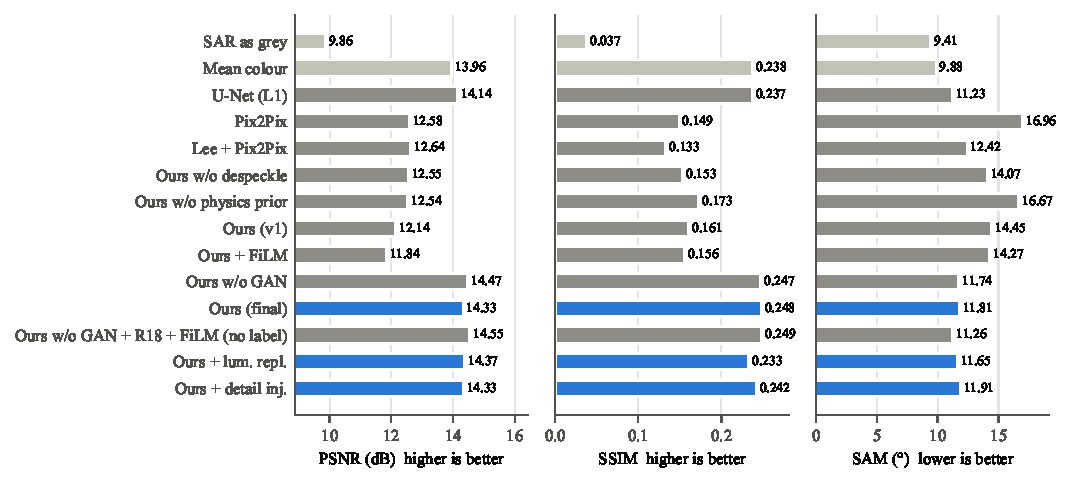
\includegraphics[width=\textwidth]{fig_comparison.pdf}
\caption{Test PSNR, SSIM and SAM for all methods. Blue: final model and its fused outputs; dark grey: baselines and ablations;
light grey: trivial floors.}
\label{fig:comparison}
\end{figure*}

\subsection{Ablation}\label{sec:ablation}
Table~\ref{tab:ablation} isolates each component.
\emph{Adversarial loss.} Removing the GAN term from our model raises PSNR by \dGanCost{}\,dB, and Pix2Pix trails the identical
U-Net trained with L1 alone by \dPixVsUnet{}\,dB. On unseen scenes the discriminator pushes the generator towards vivid but wrong
colours and creates artefacts (Fig.~\ref{fig:qual}). This is the perception--distortion trade-off~\cite{blau2018perception},
and it dominates every other design choice.
\emph{Physics prior.} Without $\mathcal{L}_{phys}$, Stage~1 is shaped only by the colorization loss and develops a strong radiometric
bias (MoR \morOursNophys). With the prior the bias disappears (MoR \morOurs, Table~\ref{tab:despeckle}).
\emph{Pretrained encoder and FiLM.} Adding both to the non-adversarial model gives the best validation L1 and the highest test
SSIM, but its test PSNR (\psnrOursRBICondNoadv{}\,dB) is slightly below that of the non-adversarial model without them
(\psnrOursNoadv{}\,dB): the two additions mainly speed up and stabilise training (Fig.~\ref{fig:train}) rather than raise
accuracy. Moreover, supplying the true terrain label at test time is \dNoLabelVsFinal{}\,dB \emph{worse} than using the ``unknown''
embedding ($p\,\pNoLabelPsnr$), even though the label helped on the validation scenes. The class-specific palettes learned from
18 training scenes therefore do not transfer reliably to new scenes. We keep the validation-selected configuration (with label)
as the final model and report the label-free result for transparency.

\begin{table*}[t]
\caption{Ablation (test set). S1: despeckling stage; $\mathcal{L}_{phys}$: physics prior; $\mathcal{L}_{s,g}$: SSIM and gradient
losses; R18: pretrained ResNet-18 encoder; FiLM: terrain conditioning. MoR: mean of ratio of the Stage~1 output (ideal 1).}
\label{tab:ablation}
\centering\footnotesize
\begin{tabular}{lcccccccccc}
\toprule
Variant & S1 & $\mathcal{L}_{phys}$ & $\mathcal{L}_{s,g}$ & GAN & R18 & FiLM & PSNR$\uparrow$ & SSIM$\uparrow$ & SAM$\downarrow$ & MoR \\
\midrule
U-Net (L1) & -- & -- & -- & -- & -- & -- & 14.14 & 0.237 & 11.23 & -- \\
Pix2Pix & -- & -- & -- & \checkmark & -- & -- & 12.58 & 0.149 & 16.96 & -- \\
Ours w/o despeckle & -- & -- & \checkmark & \checkmark & -- & -- & 12.55 & 0.153 & 14.07 & -- \\
Ours w/o physics prior & \checkmark & -- & \checkmark & \checkmark & -- & -- & 12.54 & 0.173 & 16.67 & 1.348 \\
Ours (v1) & \checkmark & \checkmark & \checkmark & \checkmark & -- & -- & 12.14 & 0.161 & 14.45 & 0.997 \\
Ours + FiLM & \checkmark & \checkmark & \checkmark & \checkmark & -- & \checkmark & 11.84 & 0.156 & 14.27 & 0.995 \\
Ours w/o GAN & \checkmark & \checkmark & \checkmark & -- & -- & -- & 14.47 & 0.247 & 11.74 & 0.998 \\
\textbf{Ours (final)} & \checkmark & \checkmark & \checkmark & -- & \checkmark & \checkmark & 14.33 & 0.248 & 11.81 & 0.986 \\
\bottomrule
\end{tabular}
\end{table*}

\subsection{Despeckling quality}
Table~\ref{tab:despeckle} compares the Stage~1 outputs with the raw SAR and the Lee filter on identical homogeneous blocks. The
Lee filter smooths most strongly (ENL \enlLee). Our Stage~1 is a mild filter (ENL \enlOursRBICondNoadv{} versus \enlRaw{} raw)
that keeps edges (EPI \epiOursRBICondNoadv) and radiometry. The stage trained without the prior \emph{lowers} ENL to \enlOursNophys, which
means it adds texture rather than removing speckle.

\begin{table}[t]
\caption{No-reference despeckling metrics (median over test tiles).}
\label{tab:despeckle}
\centering\scriptsize\setlength{\tabcolsep}{3pt}
\resizebox{\columnwidth}{!}{\begin{tabular}{lccc}
\toprule
Filter & ENL$\uparrow$ & EPI$\uparrow$ & MoR (ideal 1) \\
\midrule
Raw SAR (no filter) & 39.4 & 1.000 & 1.000 \\
Lee filter ($7{\times}7$, $L{=}40$) & 171.7 & 0.858 & 0.988 \\
Stage 1, no physics prior & 14.7 & 0.608 & 1.348 \\
Stage 1 + physics prior (v1) & 43.9 & 0.599 & 0.997 \\
Stage 1 + prior (FiLM) & 52.1 & 0.659 & 0.995 \\
Stage 1 + prior, no GAN & 49.5 & 0.624 & 0.998 \\
Stage 1 + prior, no GAN (R18+FiLM) & 54.7 & 0.903 & 0.986 \\
\bottomrule
\end{tabular}}
\end{table}

\subsection{Per-terrain results}
Table~\ref{tab:terrain} breaks the results down by class. The final model is best on barren, grassland and urban PSNR, and the
U-Net is best on agriculture. Grassland has the largest SAM for every method because one test scene contains a lake. SAR shows
it as dark, smooth backscatter, but no model renders it as water (Fig.~\ref{fig:qual}, third row).

\begin{table}[t]
\caption{Per-terrain test PSNR (dB) and SAM ($^\circ$). Bold: best per column.}
\label{tab:terrain}
\centering\scriptsize\setlength{\tabcolsep}{2.5pt}
\resizebox{\columnwidth}{!}{\begin{tabular}{lcccccccc}
\toprule
 & \multicolumn{2}{c}{Agriculture} & \multicolumn{2}{c}{Barren} & \multicolumn{2}{c}{Grassland} & \multicolumn{2}{c}{Urban} \\
 & PSNR & SAM & PSNR & SAM & PSNR & SAM & PSNR & SAM \\
\midrule
U-Net (L1) & \textbf{13.85} & 10.35 & 14.41 & 6.35 & 14.79 & 20.37 & 13.53 & 7.83 \\
Pix2Pix & 12.24 & 15.28 & 12.52 & 9.79 & 13.19 & 30.88 & 12.36 & 11.88 \\
Lee + Pix2Pix & 11.46 & 11.41 & 12.05 & 7.48 & 14.59 & \textbf{19.77} & 12.44 & 11.01 \\
Ours (final) & 13.40 & \textbf{9.14} & \textbf{14.48} & \textbf{3.90} & \textbf{15.53} & 26.61 & \textbf{13.89} & \textbf{7.58} \\
\bottomrule
\end{tabular}}
\end{table}

\begin{figure*}[t]
\centering
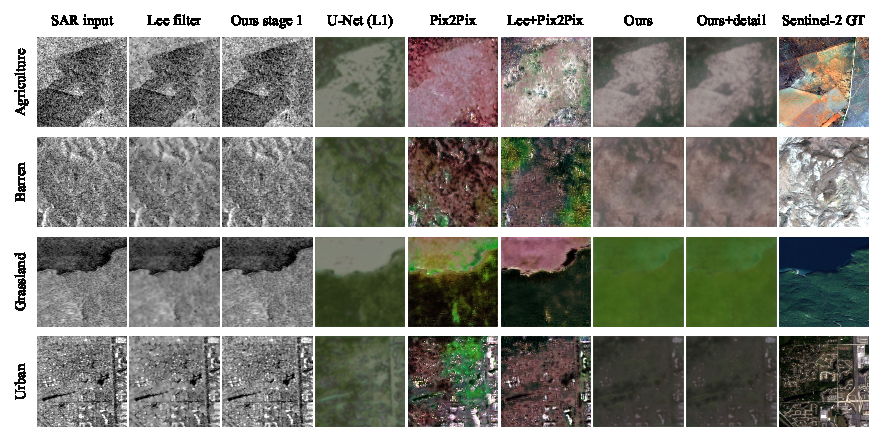
\includegraphics[width=\textwidth]{fig_qualitative.pdf}
\caption{Qualitative test results, one tile per terrain class (all scenes unseen in training). ``Ours stage 1'' is the
despeckled input of the final model. GAN-based methods hallucinate saturated colours and blob artefacts. The non-adversarial
final model produces muted but terrain-plausible palettes and misses the lake in the grassland tile.}
\label{fig:qual}
\end{figure*}

\subsection{Uncertainty}
Fig.~\ref{fig:spars} shows sparsification curves for the final model ($T{=}\mcT$, \nMC{} tiles). Removing the most uncertain
pixels does \emph{not} lower the error of the remaining pixels: the model curve stays close to random removal (AUSE \ause,
Spearman $\rho=\uncRho$). Averaging the MC passes changes PSNR by only \mcGain{}\,dB. MC-dropout variance here reflects decoder
stochasticity, not colour ambiguity, and it should not be presented as a hallucination guardrail without a calibration test of
this kind.

\begin{figure}[t]
\centering
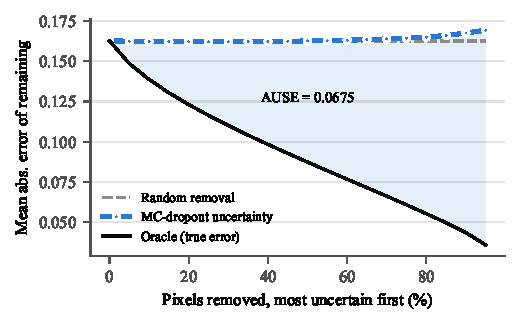
\includegraphics[width=\columnwidth]{fig_sparsification.pdf}
\caption{Sparsification curves of the final model. A useful uncertainty would follow the oracle; MC-dropout variance does not.}
\label{fig:spars}
\end{figure}

\subsection{Structure-guided fusion}
Fig.~\ref{fig:fusion} sweeps the fusion strength. Luminance replacement at the prototype setting $\alpha{=}0.7$ lowers PSNR by
about 2.6\,dB, because SAR brightness is not optical brightness. Detail injection improves edge fidelity (GMSD) at a much smaller
PSNR cost. Validation selects small strengths ($\alpha{=}\fusionAlpha$, $\beta{=}\fusionBeta$), and neither fusion yields a
meaningful fidelity gain over the raw network output (Table~\ref{tab:main}). We therefore offer fusion only as a display option.

\begin{figure}[t]
\centering
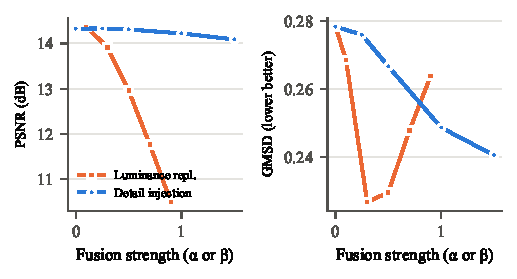
\includegraphics[width=\columnwidth]{fig_fusion.pdf}
\caption{Test PSNR and GMSD versus fusion strength (0 = no fusion).}
\label{fig:fusion}
\end{figure}

\subsection{Training dynamics and cost}
Validation curves (Fig.~\ref{fig:train}) show that the GAN-based models fluctuate strongly between checkpoints, whereas the
pretrained-encoder model is stable from the first 500 iterations. All generators have 8.3--9.6\,M parameters. Stage~1 doubles
inference time, from 15.0 to 31.5\,ms per $256{\times}256$ tile (batch 1, NVIDIA MX550), which is still interactive on a laptop
GPU.

\begin{figure}[t]
\centering
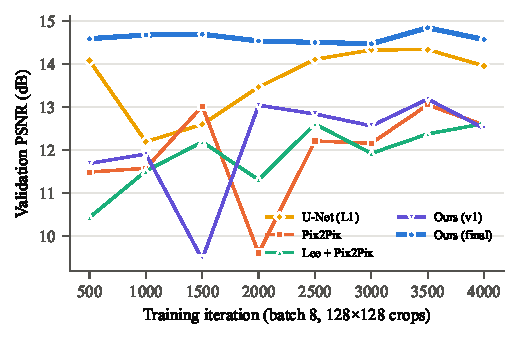
\includegraphics[width=\columnwidth]{fig_training.pdf}
\caption{Validation PSNR during training (identical budget for all models).}
\label{fig:train}
\end{figure}

\section{Limitations}
(i)~Sentinel-1 and Sentinel-2 acquisitions are not simultaneous, so pixel metrics are bounded by real scene change between
them. (ii)~The 8-bit PNG tiles are not calibrated $\sigma^0$, so the speckle model is applied to quantised backscatter.
(iii)~Only single-polarization input is used. (iv)~The budget is small (4{,}000 iterations on a 2\,GB GPU), so the absolute
numbers would likely rise with longer training, and the ranking might change. (v)~The test set has 8 scenes, so conclusions about
transfer across scenes, in particular the effect of terrain conditioning, need more scenes. (vi)~Colours are a learned estimate,
not a measurement, and should not be used for quantitative spectral analysis.

\section{Conclusion and Future Work}
We presented a physics-guided two-stage SAR colorization network and evaluated it on a leakage-free, scene-level Sentinel-1/2
benchmark with matched-budget baselines. A despeckling stage supervised only by the speckle model preserves radiometry. A
non-adversarial objective gives the best PSNR and SSIM and significantly outperforms Pix2Pix and a U-Net regressor, while a
pretrained encoder mainly makes training faster and more stable. The absolute gains over trivial predictors are small, and terrain conditioning, MC-dropout uncertainty and SAR
luminance fusion did not deliver the commonly assumed benefits. We consider these negative results as useful as the positive
ones. Future work will add dual-polarization (VV+VH) and multi-temporal inputs, train longer on larger scene sets, test
uncertainty methods that are calibrated by construction (e.g.\ deep ensembles or conformal prediction), and investigate
conditional diffusion models~\cite{rombach2022ldm}, Swin Transformer encoders~\cite{liu2021swin} and perceptual metrics such as
LPIPS.

\section*{Acknowledgment}
Sentinel-1 and Sentinel-2 data are provided by the European Space Agency through the Copernicus programme.

\bibliographystyle{IEEEtran}
\bibliography{refs}

\end{document}
